%% LyX 2.3.0 created this file.  For more info, see http://www.lyx.org/.
%% Do not edit unless you really know what you are doing.
\documentclass[english]{article}
\usepackage[T1]{fontenc}
\usepackage[latin9]{inputenc}
\usepackage{geometry}
\geometry{verbose,tmargin=2cm,bmargin=2cm,lmargin=2cm,rmargin=2cm,headheight=2cm,headsep=2cm,footskip=2cm}
\usepackage{float}
\usepackage{booktabs}
\usepackage{textcomp}
\usepackage{amstext}
\usepackage{graphicx}

\makeatletter

%%%%%%%%%%%%%%%%%%%%%%%%%%%%%% LyX specific LaTeX commands.
%% Because html converters don't know tabularnewline
\providecommand{\tabularnewline}{\\}

\makeatother

\usepackage{babel}
\begin{document}

\section*{Ejercicio 4 }

Se desea realizar un circuito que convierta un numero binario de 4
bits en su complemento a dos.

\textbullet{} Exprese el valor de cada bit de salida en funcion de
los minterminos de los bits de entrada.

\textbullet{} Exprese el valor de cada bit de salida en forma simplificada. 

\textbullet{} Dibuje el circuito logico resultante utilizando compuertas
AND, OR, NOT. 

\textbullet{} Implemente el circuito resultante en Verilog.

~

Para obtener el complemento a dos de un numero binario se invierte
el valor de cada una de sus cifras, es decir, se realiza el complemento
a uno, y luego se le suma uno al numero resultante de la inversion. 

Su utilidad principal se encuentra en las operaciones matematicas
con numeros binarios. En particular, la resta de numeros binarios
se facilita enormemente utilizando el complemento a dos: la resta
de dos numeros binarios puede obtenerse sumando al minuendo el complemento
a dos del sustraendo. 

~

Ademas, llamaremos mintermino $m_{i}$ a aquel que se forma multiplicando
(AND logico) todas las variables, negando aquellas que valen 0 en
la combinacion para la cual queremos que el mintermino valga 1. Para
N variables booleanas, existen $2^{N}$ mintermino, uno para cada
posible combinacion de ellas.

~

A continuacion se realiza la tabla de verdad para un numero binario
de 4 bits. Donde a cada numero binario ($x_{1}$$x_{2}$$x_{3}$$x_{4}$)
le corresponde su respectivo complemento a dos a la salida ($f_{1}f_{2}f_{3}f_{4}$).

\begin{table}[H]
\begin{centering}
\begin{tabular}{cccc}
\toprule 
$x_{1}$ & $x_{2}$ & $x_{3}$ & $x_{4}$\tabularnewline
\midrule
\midrule 
0 & 0 & 0 & 0\tabularnewline
\midrule 
0 & 0 & 0 & 1\tabularnewline
\midrule 
0 & 0 & 1 & 0\tabularnewline
\midrule 
0 & 0 & 1 & 1\tabularnewline
\midrule 
0 & 1 & 0 & 0\tabularnewline
\midrule 
0 & 1 & 0 & 1\tabularnewline
\midrule 
0 & 1 & 1 & 0\tabularnewline
\midrule 
0 & 1 & 1 & 1\tabularnewline
\midrule 
1 & 0 & 0 & 0\tabularnewline
\midrule 
1 & 0 & 0 & 1\tabularnewline
\midrule 
1 & 0 & 1 & 0\tabularnewline
\midrule 
1 & 0 & 1 & 1\tabularnewline
\midrule 
1 & 1 & 0 & 0\tabularnewline
\midrule 
1 & 1 & 0 & 1\tabularnewline
\midrule 
1 & 1 & 1 & 0\tabularnewline
\midrule 
1 & 1 & 1 & 1\tabularnewline
\bottomrule
\end{tabular}%
\begin{tabular}{cccc}
\toprule 
$f_{1}$ & $f_{2}$ & $f_{3}$ & $f_{4}$\tabularnewline
\midrule
\midrule 
0 & 0 & 0 & 0\tabularnewline
\midrule 
1 & 1 & 1 & 1\tabularnewline
\midrule 
1 & 1 & 1 & 0\tabularnewline
\midrule 
1 & 1 & 0 & 1\tabularnewline
\midrule 
1 & 1 & 0 & 0\tabularnewline
\midrule 
1 & 0 & 1 & 1\tabularnewline
\midrule 
1 & 0 & 1 & 0\tabularnewline
\midrule 
1 & 0 & 0 & 1\tabularnewline
\midrule 
1 & 0 & 0 & 0\tabularnewline
\midrule 
0 & 1 & 1 & 1\tabularnewline
\midrule 
0 & 1 & 1 & 0\tabularnewline
\midrule 
0 & 1 & 0 & 1\tabularnewline
\midrule 
0 & 1 & 0 & 0\tabularnewline
\midrule 
0 & 0 & 1 & 1\tabularnewline
\midrule 
0 & 0 & 1 & 0\tabularnewline
\midrule 
0 & 0 & 0 & 1\tabularnewline
\bottomrule
\end{tabular}{\small{}}%
\begin{tabular}{c}
\toprule 
$m_{i}$\tabularnewline
\midrule
\midrule 
{\small{}$m_{0}$}\tabularnewline
\midrule 
{\small{}$m_{1}$}\tabularnewline
\midrule 
{\small{}$m_{2}$}\tabularnewline
\midrule 
{\small{}$m_{3}$}\tabularnewline
\midrule 
{\small{}$m_{4}$}\tabularnewline
\midrule 
{\small{}$m_{5}$}\tabularnewline
\midrule 
{\small{}$m_{6}$}\tabularnewline
\midrule 
{\small{}$m_{7}$}\tabularnewline
\midrule 
{\small{}$m_{8}$}\tabularnewline
\midrule 
{\small{}$m_{9}$}\tabularnewline
\midrule 
{\small{}$m_{10}$}\tabularnewline
\midrule 
{\small{}$m_{11}$}\tabularnewline
\midrule 
{\small{}$m_{12}$}\tabularnewline
\midrule 
{\small{}$m_{13}$}\tabularnewline
\midrule 
{\small{}$m_{14}$}\tabularnewline
\midrule 
{\small{}$m_{15}$}\tabularnewline
\bottomrule
\end{tabular}{\small\par}
\par\end{centering}
\caption{Complemento a dos $(f_{1}$$f_{2}$$f_{3}$$f_{4}$) del bit de entrada
($x_{1}$$x_{2}$$x_{3}$$x_{4}$) }

\end{table}

Se expresa la salida como funcion de los minterminos. Para expresar
la funcion en minterminos tomamos donde la funcion sea 1 y unimos
los minterminos con sumas:
\begin{center}
$f_{1}(m_{i})=m_{1}+m_{2}+m_{3}+m_{4}+m_{5}+m_{6}+m_{7}+m_{8}$
\par\end{center}

\begin{center}
$f_{2}(m_{i})=m_{1}+m_{2}+m_{3}+m_{4}+m_{9}+m_{10}+m_{11}+m_{12}$
\par\end{center}

\begin{center}
$f_{3}(m_{i})=m_{1}+m_{2}+m_{5}+m_{6}+m_{9}+m_{10}+m_{13}+m_{14}$
\par\end{center}

\begin{center}
$f_{4}(m_{i})=m_{1}+m_{3}+m_{5}+m_{7}+m_{9}+m_{11}+m_{13}+m_{15}$
\par\end{center}

Se reemplaza por los valores de entrada,

~

$f_{1}(x_{1},x_{2},x_{3},x_{4})=\overline{x_{1}}\overline{x_{2}}\overline{x_{3}}x_{4}+\overline{x_{1}}\overline{x_{2}}x_{3}\overline{x_{4}}+\overline{x_{1}}\overline{x_{2}}x_{3}x_{4}+\overline{x_{1}}x_{2}\overline{x_{3}}\overline{x_{4}}+\overline{x_{1}}x_{2}\overline{x_{3}}x_{4}+\overline{x_{1}}x_{2}x_{3}\overline{x_{4}}+\overline{x_{1}}x_{2}x_{3}x_{4}+x_{1}\overline{x_{2}}\overline{x_{3}}\overline{x_{4}}$

$f_{2}(x_{1},x_{2},x_{3},x_{4})=\overline{x_{1}}\overline{x_{2}}\overline{x_{3}}x_{4}+\overline{x_{1}}\overline{x_{2}}x_{3}\overline{x_{4}}+\overline{x_{1}}\overline{x_{2}}x_{3}x_{4}+\overline{x_{1}}x_{2}\overline{x_{3}}\overline{x_{4}}+x_{1}\overline{\text{\ensuremath{x_{2}}}}\overline{x_{3}}x_{4}+x_{1}\overline{x_{2}}x_{3}\overline{x_{4}}+x_{1}\overline{x_{2}}x_{3}x_{4}+x_{1}x_{2}\overline{x_{3}}\overline{x_{4}}$

$f_{3}(x_{1},x_{2},x_{3},x_{4})=\overline{x_{1}}\overline{x_{2}}\overline{x_{3}}x_{4}+\overline{x_{1}}\overline{x_{2}}x_{3}\overline{x_{4}}+\overline{x_{1}}x_{2}\overline{x_{3}}x_{4}+\overline{x_{1}}x_{2}x_{3}\overline{x_{4}}+x_{1}\overline{\text{\ensuremath{x_{2}}}}\overline{x_{3}}x_{4}+x_{1}\overline{x_{2}}x_{3}\overline{x_{4}}+x_{1}x_{2}\overline{\text{\ensuremath{x_{3}}}}x_{4}+x_{1}x_{2}x_{3}\overline{x_{4}}$

$f_{4}(x_{1},x_{2},x_{3},x_{4})=\overline{x_{1}}\overline{x_{2}}\overline{x_{3}}x_{4}+\overline{x_{1}}\overline{x_{2}}x_{3}x_{4}+\overline{x_{1}}x_{2}\overline{x_{3}}x_{4}+\overline{x_{1}}x_{2}x_{3}x_{4}+x_{1}\overline{\text{\ensuremath{x_{2}}}}\overline{x_{3}}x_{4}+x_{1}\overline{x_{2}}x_{3}x_{4}+x_{1}x_{2}\overline{\text{\ensuremath{x_{3}}}}x_{4}+x_{1}x_{2}x_{3}x_{4}$

~

Finalmente, utilizando mapas de Karnaugh, se simplifican las ecuaciones.
Los mapas de Karnaugh reducen la necesidad de hacer calculos extensos
para la simplificacion de expresiones booleanas.

El mapa de Karnaugh consiste en una representacion bidimensional de
la tabla de verdad de la funcion a simplificar. Puesto que la tabla
de verdad de una funcion de N variables posee $2^{N}$ filas, el mapa
K correspondiente debe poseer tambien $2^{N}$ cuadrados. Las variables
de la expresion son ordenadas en funcion de su peso y siguiendo el
codigo Gray, de manera que solo una de las variables varia entre celdas
adyacentes. La transferencia de los terminos de la tabla de verdad
al mapa de Karnaugh se realiza de forma directa, albergando un 0 o
un 1, dependiendo del valor que toma la funcion en cada fila.

~

En la Figura 1 podemos observar el mapa de Karnaugh de $f_{1}$ con
cuatro conjuntos encerrados por distintos colores:

\textbullet{} La funcion del conjunto amarillo se produce porque se
observa que ninguna $x_{i}$ varia durante su conjunto. Como $x_{2},x_{3}$
y $x_{4}$ no varian pero valen 0, entonces obtenemos como funcion
del conjunto $x_{1}\overline{x_{2}}\overline{x_{3}}\overline{x_{4}}.$

\textbullet{} La funcion del conjunto rojo se produce al observar
que $x_{1}$ y $x_{2}$ no varian. Sin embargo, como $x_{1}$es cero,
obtenemos como funcion del conjunto $\overline{x_{1}}x_{2}.$

\textbullet{} En el caso del conjunto verde, $x_{1}$ y $x_{3}$ no
varian pero $x_{1}$ es cero, por lo que resulta $\overline{x_{1}}x_{3}$.

\textbullet{} Finalmente, en el conjunto azul, $x_{1}$ y $x_{4}$
no varian pero $x_{1}$ es cero, por lo que resulta $\overline{x_{1}}x_{4}$.

De esta manera,
\begin{center}
$f_{1}(x_{1},x_{2},x_{3},x_{4})=x_{1}\overline{x_{2}}\overline{x_{3}}\overline{x_{4}}+\overline{x_{1}}x_{2}+\overline{x_{1}}x_{3}+\overline{x_{1}}x_{4}=x_{1}\overline{x_{2}}\overline{x_{3}}\overline{x_{4}}+\overline{x_{1}}(x_{2}+x_{3}+x_{4})$
\par\end{center}

~

\begin{figure}[H]
\begin{centering}
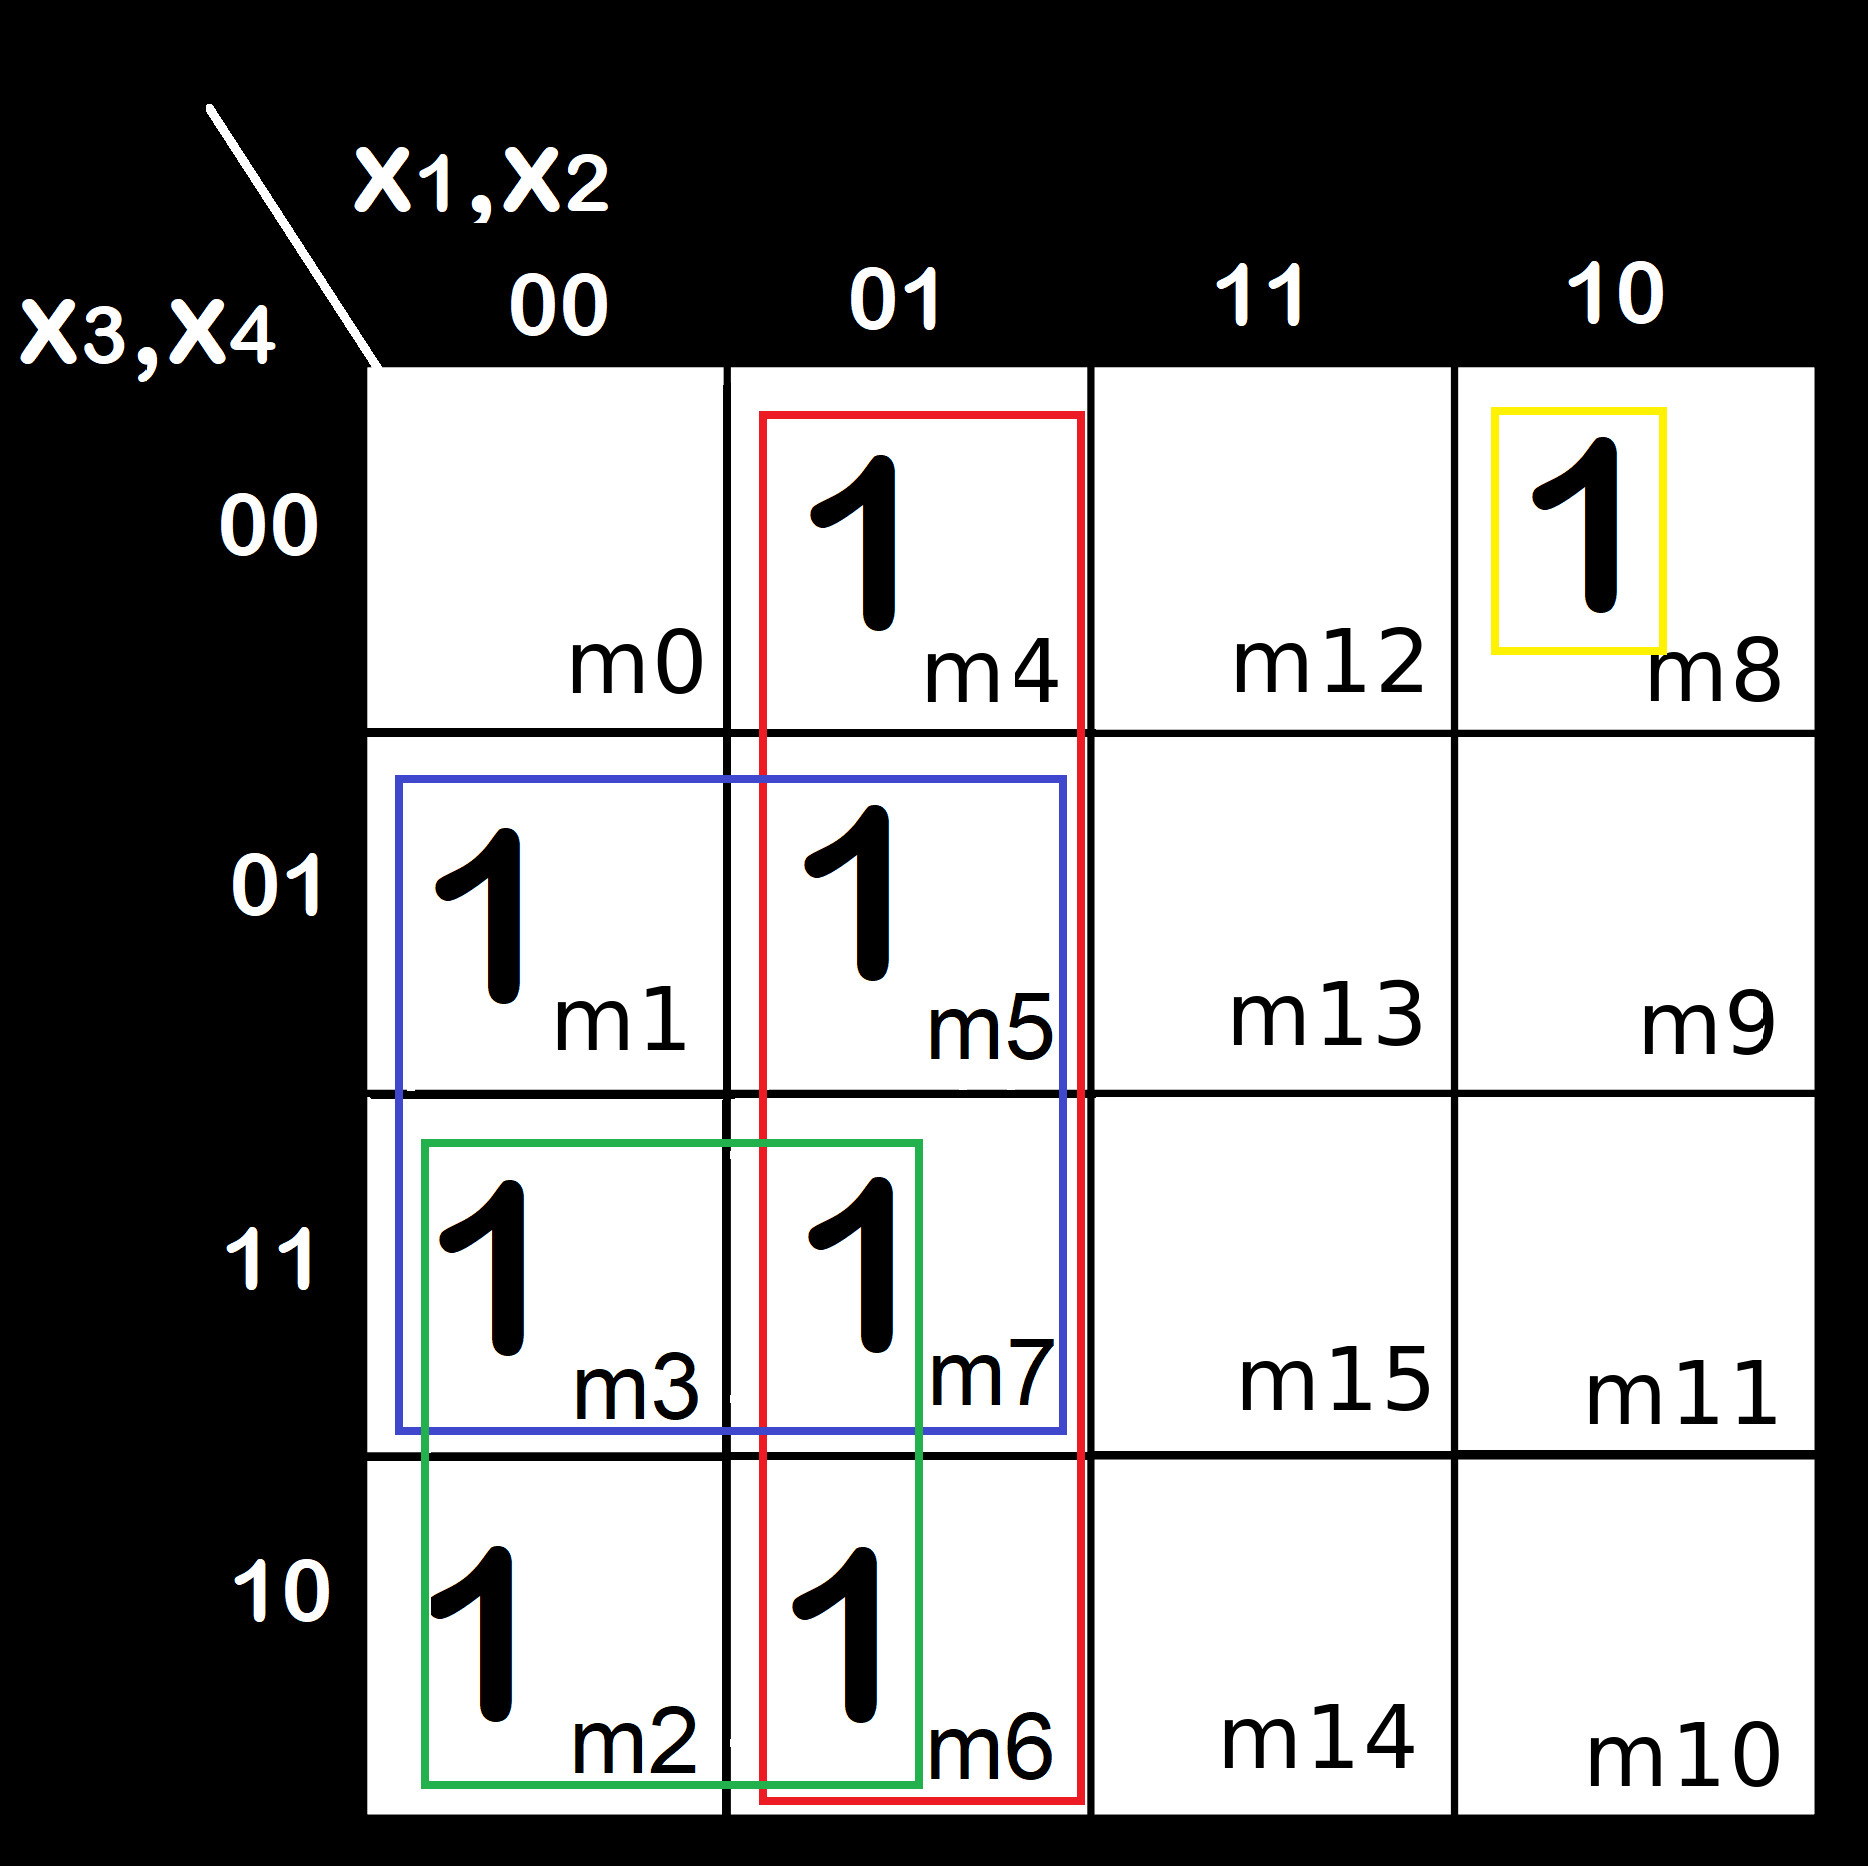
\includegraphics[scale=0.3]{karno1}
\par\end{centering}
\caption{Mapa de Karnaugh $f_{1}(x_{1},x_{2},x_{3},x_{4})$}

\end{figure}

\pagebreak{}

El analisis para los siguientes casos se realiza de la misma manera,
pero no sera detallado. Solo se procedera a mostrar las funciones
simplificadas y sus respectivos mapas de Karnaugh.

~

Para $f_{2}$,
\begin{center}
$f_{2}(x_{1},x_{2},x_{3},x_{4})=x_{2}\overline{x_{3}}\overline{x_{4}}+\overline{\text{\ensuremath{x_{2}}}}x_{3}+\overline{x_{2}}x_{4}=x_{2}\overline{x_{3}}\overline{x_{4}}+\overline{\text{\ensuremath{x_{2}}}}(x_{3}+x_{4})$
\par\end{center}

\begin{figure}[H]
\begin{centering}
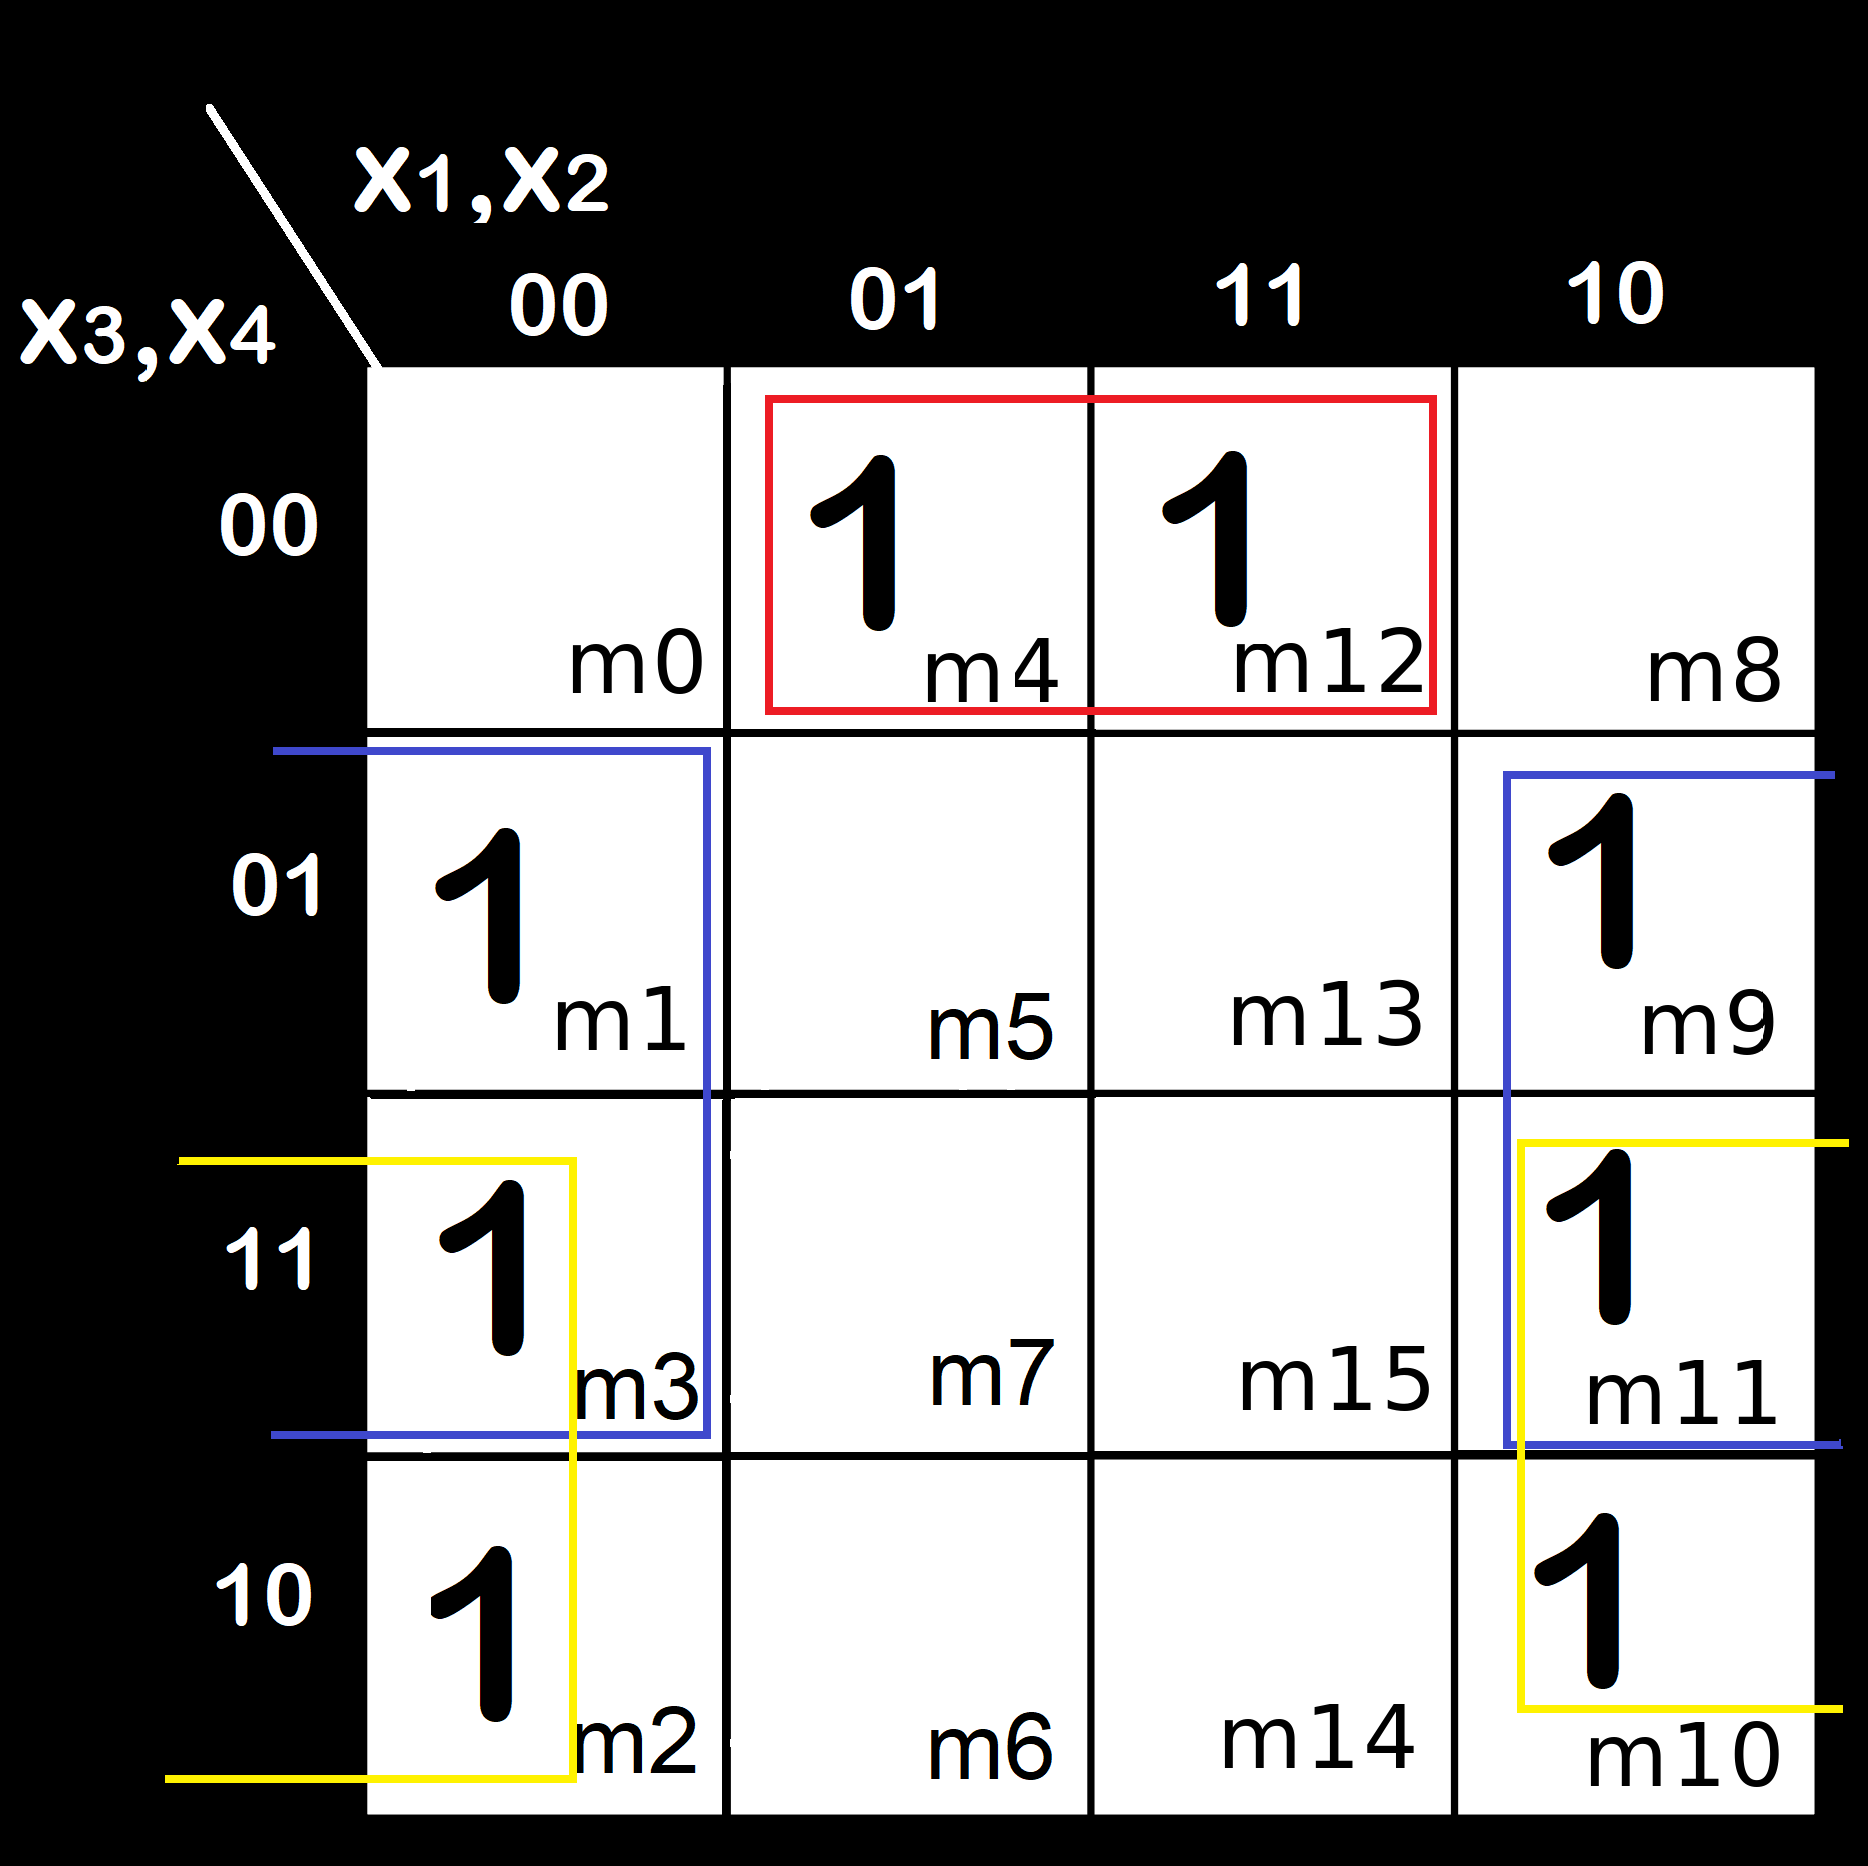
\includegraphics[scale=0.3]{karno2}
\par\end{centering}
\caption{Mapa de Karnaugh $f_{2}(x_{1},x_{2},x_{3},x_{4})$}
\end{figure}

~

~

~

Para $f_{3}$,
\begin{center}
$f_{3}(x_{1},x_{2},x_{3},x_{4})=\overline{x_{3}}x_{4}+x_{3}\overline{x_{4}}$
\par\end{center}

\begin{figure}[H]
\begin{centering}
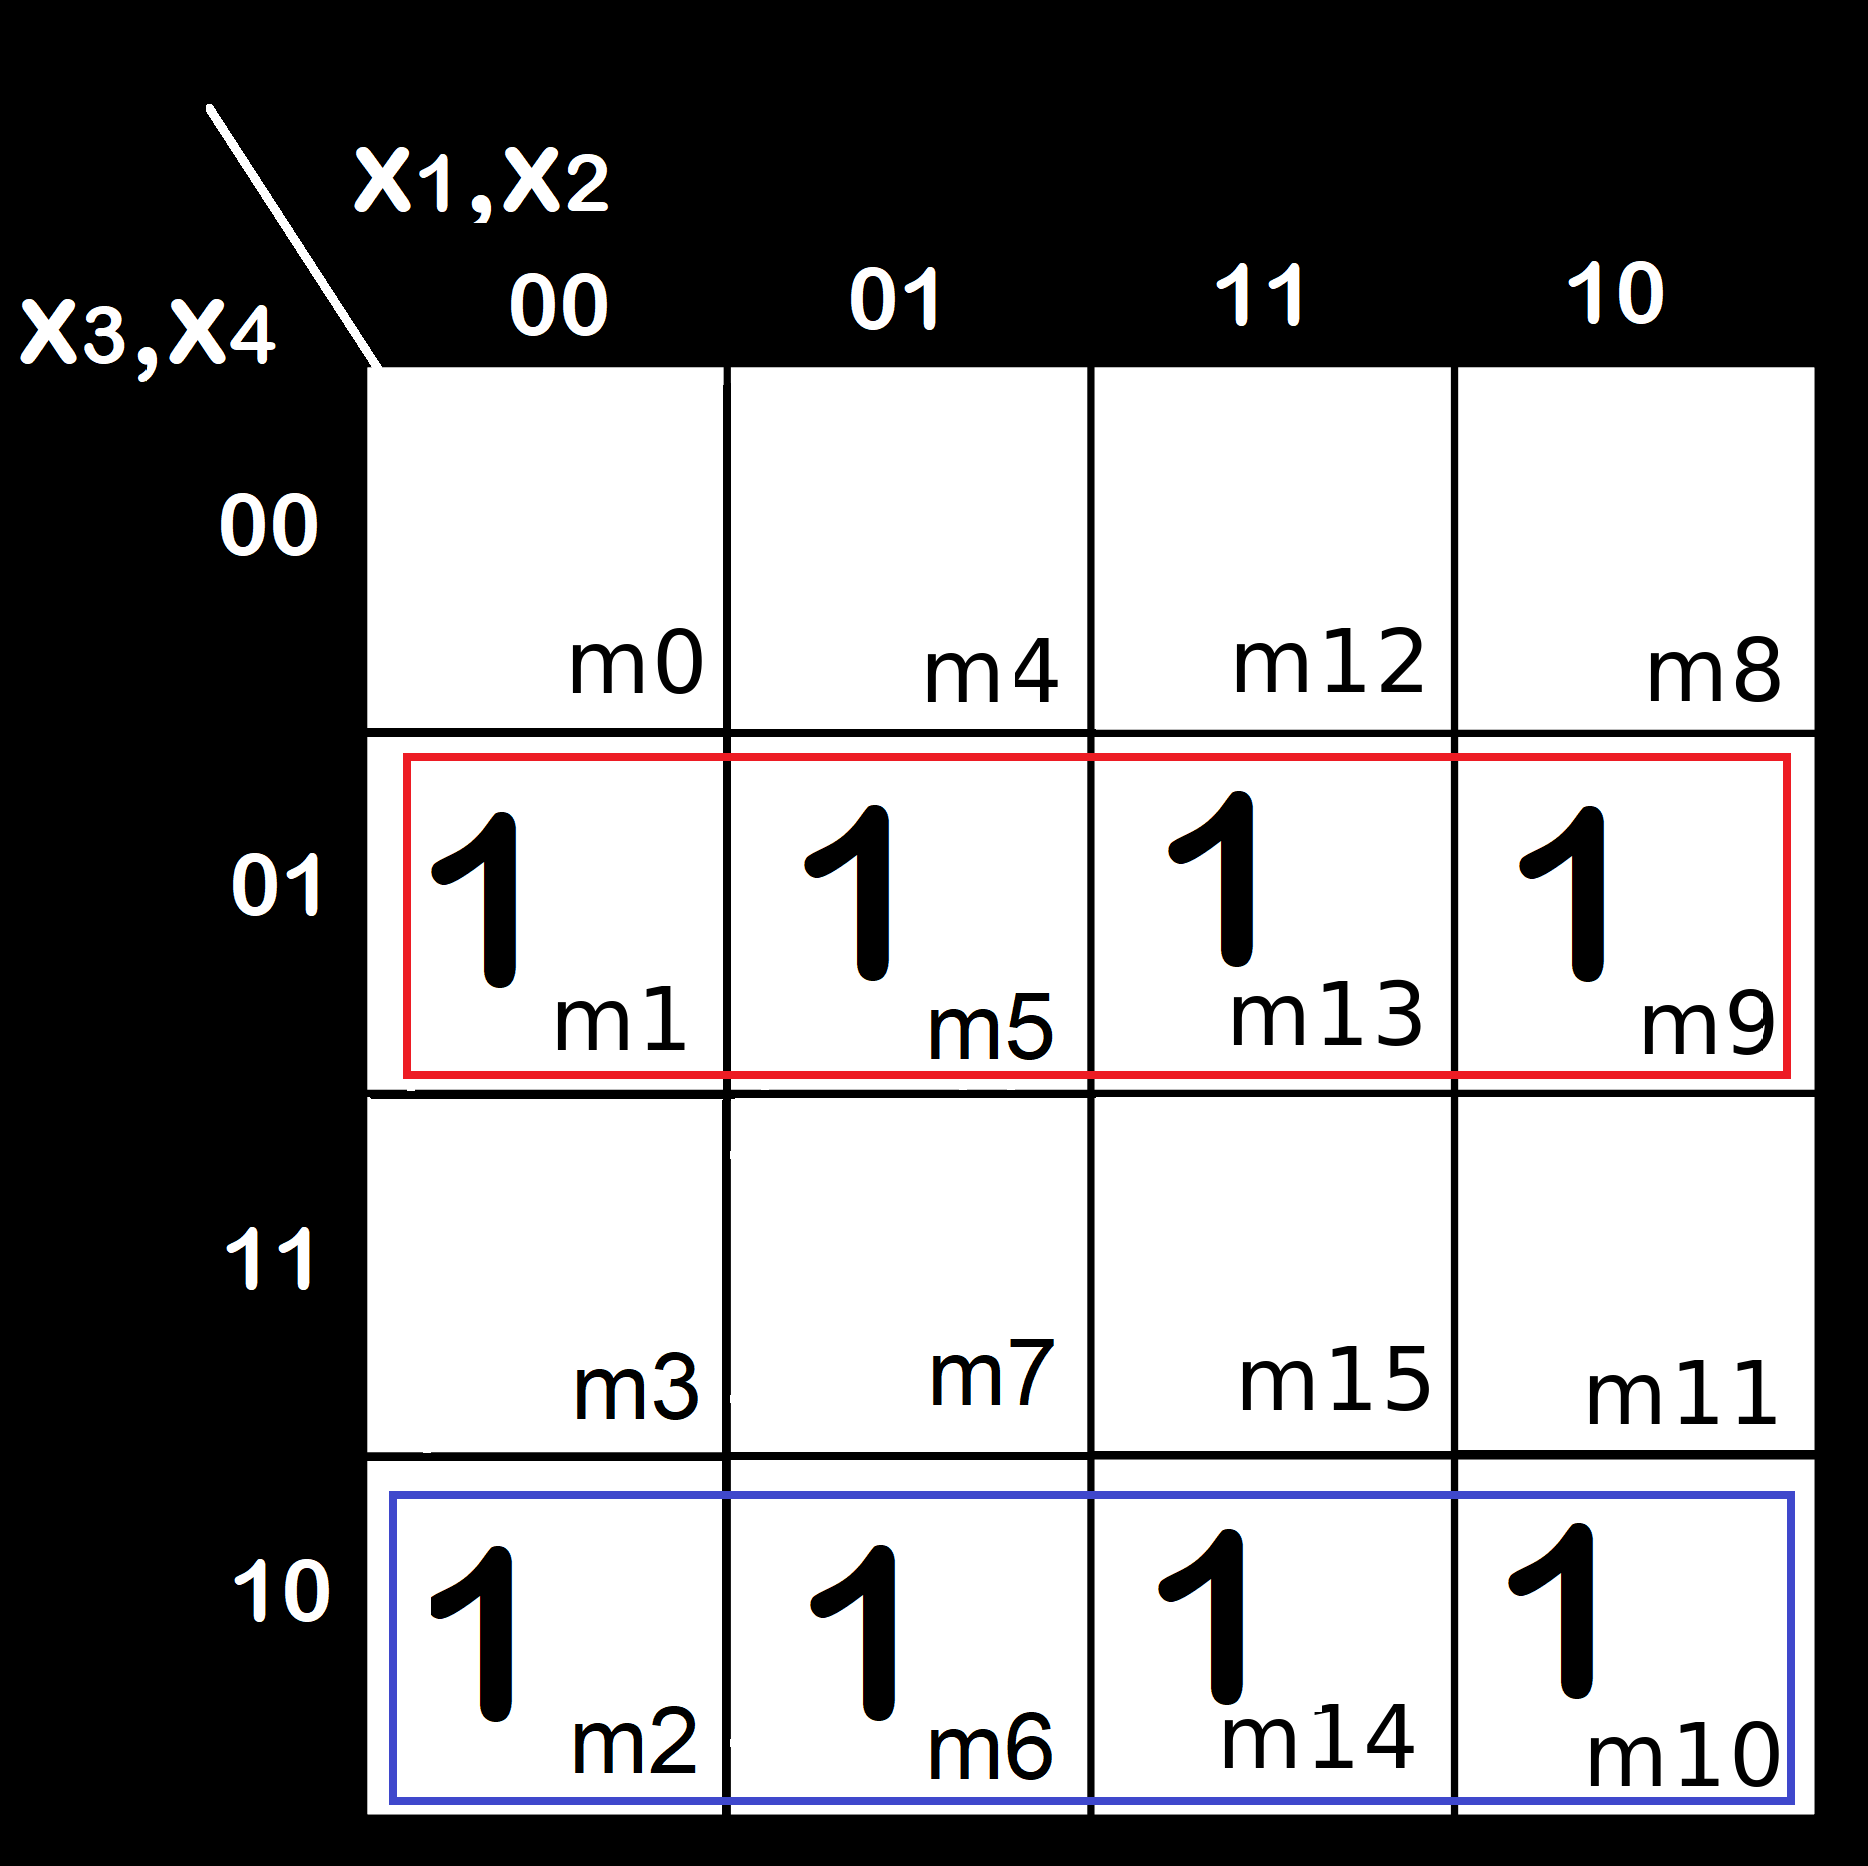
\includegraphics[scale=0.3]{karno3}
\par\end{centering}
\caption{Mapa de Karnaugh $f_{3}(x_{1},x_{2},x_{3},x_{4})$}
\end{figure}

\pagebreak{}

Para $f_{4}$,
\begin{center}
$f_{4}(x_{1},x_{2},x_{3},x_{4})=x_{4}$
\par\end{center}

\begin{figure}[H]
\begin{centering}
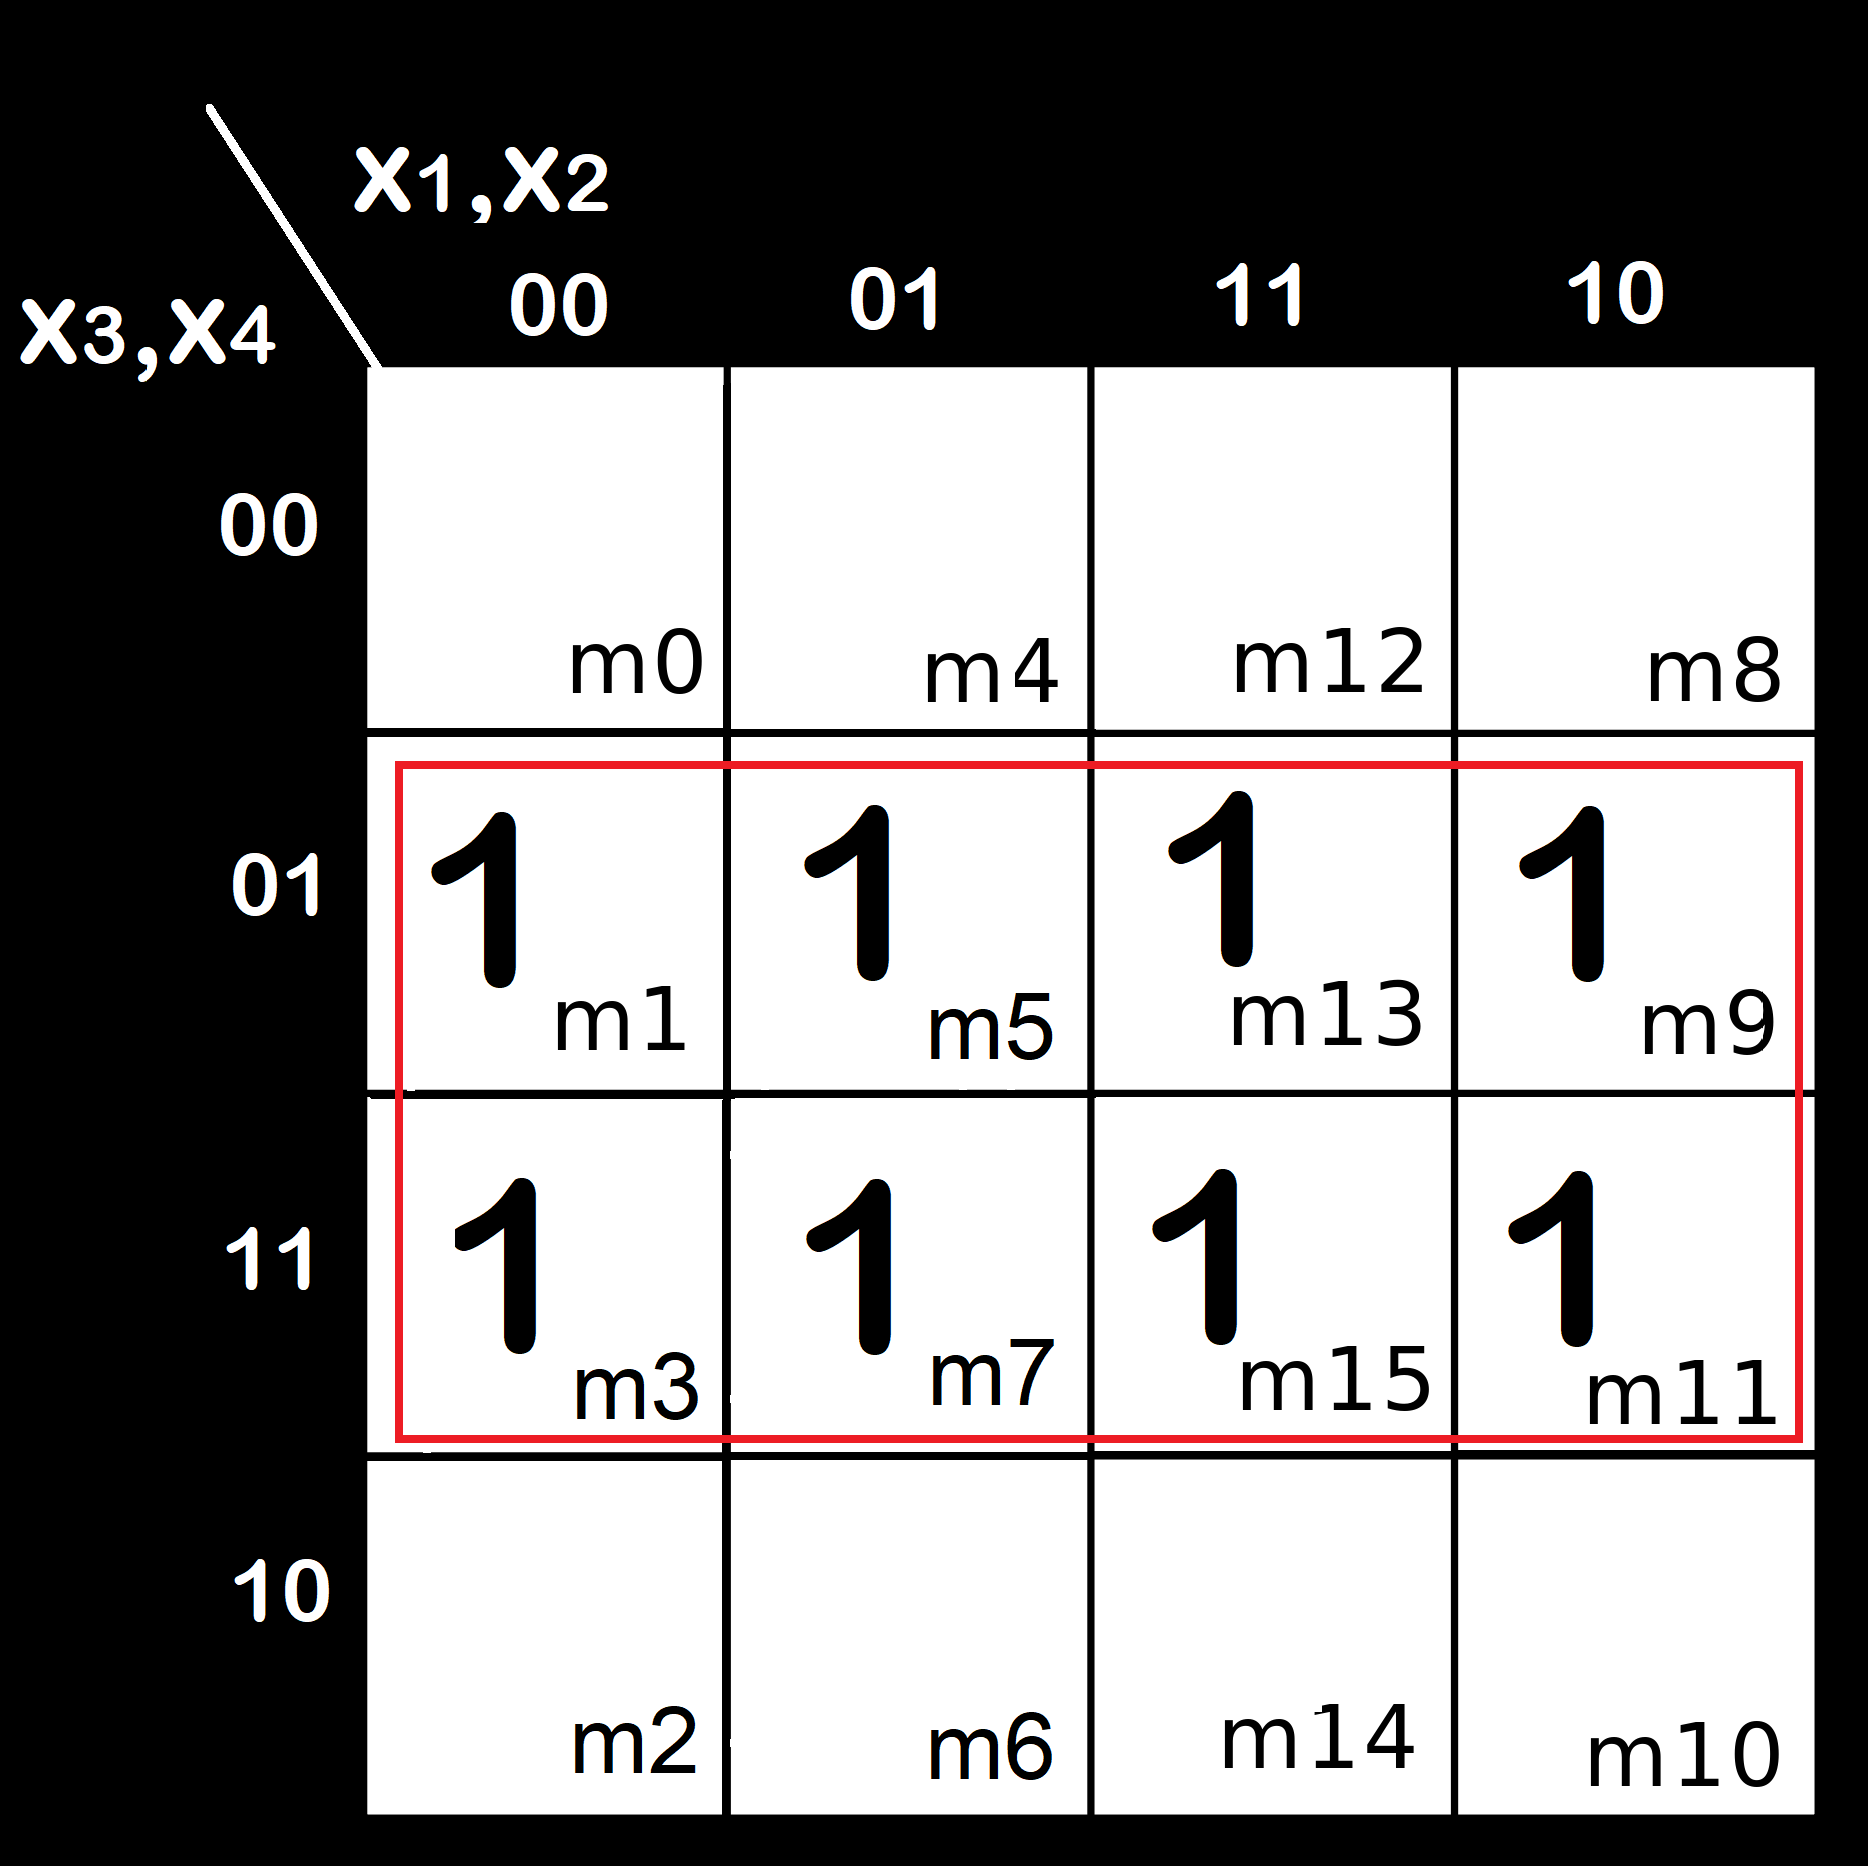
\includegraphics[scale=0.3]{karno4}
\par\end{centering}
\caption{Mapa de Karnaugh $f_{4}(x_{1},x_{2},x_{3},x_{4})$}

\end{figure}

El circuito logico resultante se muestra en la Figura 5, donde los
Xi corresponden a la entrada y los Fi a la salida del circuito. Respetando
la consigna, solo se utilizaron compuestas NOT, AND y OR.

~

\begin{figure}[H]
\begin{centering}
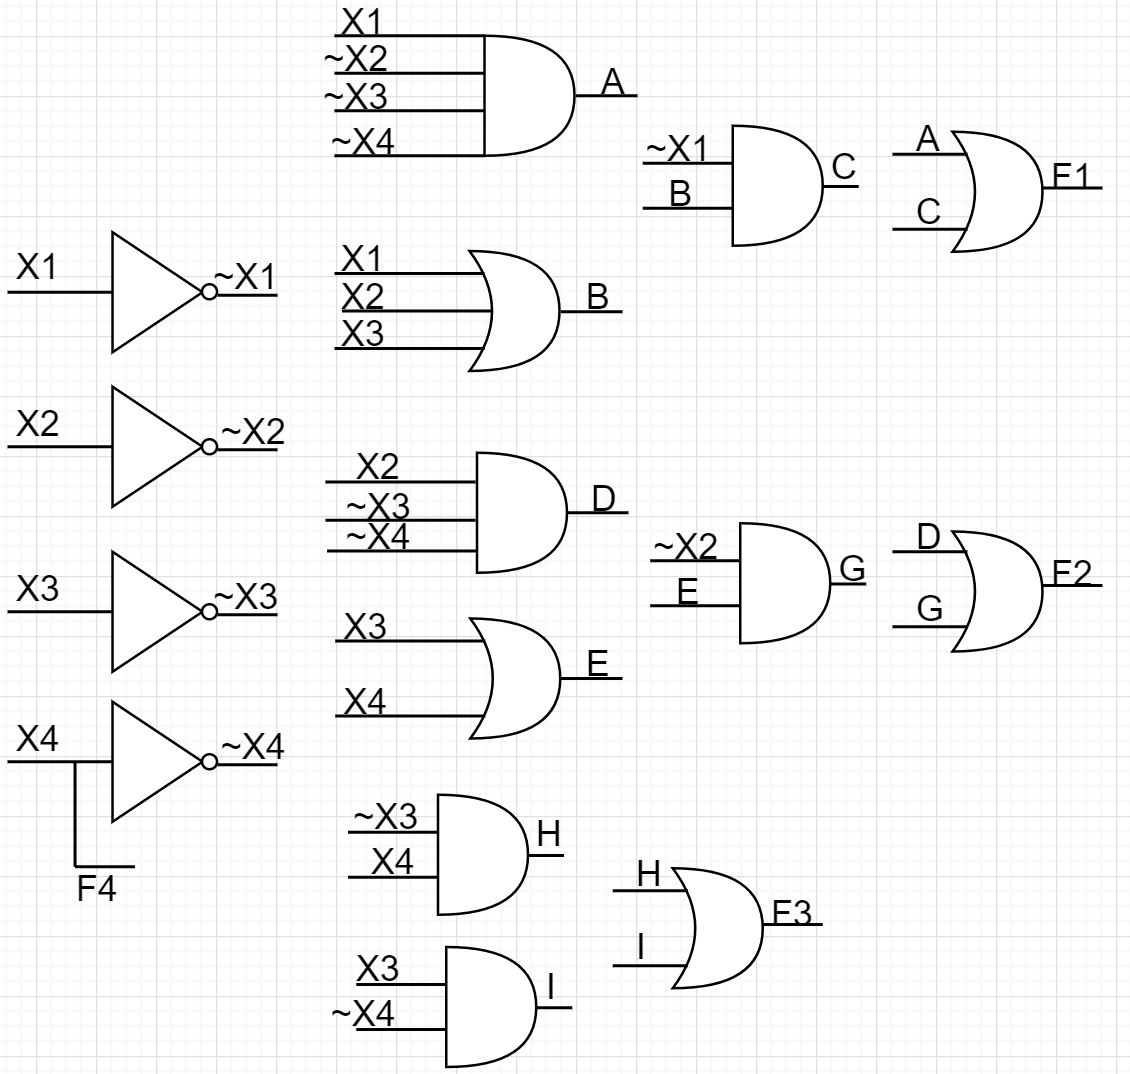
\includegraphics[scale=1.1]{gateTOTAL}
\par\end{centering}
\caption{Circuito resultante realizado en draw.io}

\end{figure}

\end{document}
